\documentclass[tikz,border=3.14mm]{standalone}
\usepackage{tikz}
\usetikzlibrary{calc}

\begin{document}
    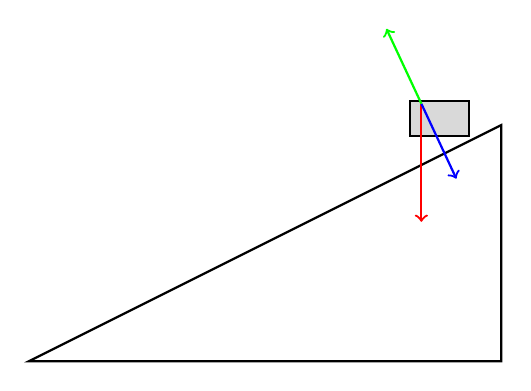
\begin{tikzpicture}[scale=1.5]
        % Incline
        \draw[thick] (0,0) -- (4,0) -- (4,2) -- cycle;
        
        % Block
        \filldraw[fill=gray!30, draw=black, thick] ($(4,2)+(165:0.8)$) rectangle ++(0.5, -0.3);
        
        % Vectors
        \draw[->, red, thick] ($(4,2)+(165:0.7)$) -- ++(0,-1); % gravitational force
        \draw[->, blue, thick] ($(4,2)+(165:0.7)$) -- ++(-65:0.7); % normal force 
        \draw[->, green,thick] ($(4,2)+(165:0.7)$) -- ++(180-65:0.7); % frictional force       
    \end{tikzpicture}
\end{document}